% wording - markets or investors
\documentclass[11pt, oneside, article]{memoir}\usepackage[]{graphicx}\usepackage[]{color}
%% maxwidth is the original width if it is less than linewidth
%% otherwise use linewidth (to make sure the graphics do not exceed the margin)
\makeatletter
\def\maxwidth{ %
  \ifdim\Gin@nat@width>\linewidth
    \linewidth
  \else
    \Gin@nat@width
  \fi
}
\makeatother

\definecolor{fgcolor}{rgb}{0.345, 0.345, 0.345}
\newcommand{\hlnum}[1]{\textcolor[rgb]{0.686,0.059,0.569}{#1}}%
\newcommand{\hlstr}[1]{\textcolor[rgb]{0.192,0.494,0.8}{#1}}%
\newcommand{\hlcom}[1]{\textcolor[rgb]{0.678,0.584,0.686}{\textit{#1}}}%
\newcommand{\hlopt}[1]{\textcolor[rgb]{0,0,0}{#1}}%
\newcommand{\hlstd}[1]{\textcolor[rgb]{0.345,0.345,0.345}{#1}}%
\newcommand{\hlkwa}[1]{\textcolor[rgb]{0.161,0.373,0.58}{\textbf{#1}}}%
\newcommand{\hlkwb}[1]{\textcolor[rgb]{0.69,0.353,0.396}{#1}}%
\newcommand{\hlkwc}[1]{\textcolor[rgb]{0.333,0.667,0.333}{#1}}%
\newcommand{\hlkwd}[1]{\textcolor[rgb]{0.737,0.353,0.396}{\textbf{#1}}}%

\usepackage{framed}
\makeatletter
\newenvironment{kframe}{%
 \def\at@end@of@kframe{}%
 \ifinner\ifhmode%
  \def\at@end@of@kframe{\end{minipage}}%
  \begin{minipage}{\columnwidth}%
 \fi\fi%
 \def\FrameCommand##1{\hskip\@totalleftmargin \hskip-\fboxsep
 \colorbox{shadecolor}{##1}\hskip-\fboxsep
     % There is no \\@totalrightmargin, so:
     \hskip-\linewidth \hskip-\@totalleftmargin \hskip\columnwidth}%
 \MakeFramed {\advance\hsize-\width
   \@totalleftmargin\z@ \linewidth\hsize
   \@setminipage}}%
 {\par\unskip\endMakeFramed%
 \at@end@of@kframe}
\makeatother

\definecolor{shadecolor}{rgb}{.97, .97, .97}
\definecolor{messagecolor}{rgb}{0, 0, 0}
\definecolor{warningcolor}{rgb}{1, 0, 1}
\definecolor{errorcolor}{rgb}{1, 0, 0}
\newenvironment{knitrout}{}{} % an empty environment to be redefined in TeX

\usepackage{alltt}

\usepackage[]{xcolor}
\definecolor{light-gray}{gray}{0.66}
\definecolor{dkred}{rgb}{0.5,0,0}
\definecolor{dkblue}{rgb}{0,0,0.5}

\usepackage{graphicx}
\usepackage{amsmath}
\usepackage{comment}
\usepackage{rotating}
\usepackage{todonotes}

\raggedyright
\counterwithout{section}{chapter}
\setcounter{secnumdepth}{2}

\abstractrunin
\abslabeldelim{:\quad}

% Floats
\setfloatadjustment{figure}{\centerfloat}
\setfloatadjustment{table}{\scriptsize\centering\sffamily}
\captionnamefont{\sffamily\itshape\footnotesize}
\captiontitlefont{\sffamily\footnotesize}

\usepackage[section]{placeins}


\usepackage{fontspec,xltxtra,xunicode}
\defaultfontfeatures{Mapping=tex-text}
\setmainfont[Numbers=OldStyle]{Linux Libertine O}
\setsansfont[]{Linux Biolinum O}
\setmonofont[Scale=MatchLowercase]{Linux Libertine Mono O}
\setmonofont[Scale=MatchLowercase]{DejaVu Sans Mono}
\usepackage[math-style=TeX]{unicode-math}
\setmathfont{xits-math.otf}

\usepackage[]{titlesec}
\titleformat{\section}[hang]{\color{dkred}\Large\bfseries\sffamily}{\thesection}{1em}{}{}
\titlespacing*{\section}{0em}{1.5em}{0.5em}

\titleformat{\subsection}[hang]{\large\itshape}{\addfontfeatures{Numbers=OldStyle}\thesubsection}{1em}{}
\titlespacing*{\subsection}{0em}{1.5em}{0.5em}

\titleformat{\subsubsection}[runin]{\normalsize\bfseries}{\addfontfeatures{Numbers=OldStyle}\thesubsubsection}{1em}{}[:]

\usepackage[style=authoryear,doi=false,isbn=false,backend=biber,%
            backref=true,maxbibnames=10,hyperref=true,%
            dateabbrev=false,uniquename=false]{biblatex}
\ExecuteBibliographyOptions{url=false}
\ExecuteBibliographyOptions{doi=false}
\newbibmacro{string+url}[1]{%
 \iffieldundef{doi}{\iffieldundef{url}{#1}{\href{\thefield{url}}{#1}}}{\href{http://dx.doi.org/\thefield{doi}}{#1}}}
\DeclareFieldFormat{title}{\usebibmacro{string+url}{\mkbibemph{#1}}}
\DeclareFieldFormat[article]{title}{\usebibmacro{string+url}{\mkbibquote{#1}}}
\DeclareFieldFormat[misc]{title}{\usebibmacro{string+url}{\mkbibemph{#1}}}
\DeclareFieldFormat[book]{title}{\usebibmacro{string+url}{\mkbibemph{#1}}}
\AtEveryBibitem{\clearlist{language}}

\bibliography{local.bib}

\newcommand{\email}[1]{\href{mailto:#1}{\normalfont\texttt{#1}}}

% Programming Languages
\newcommand{\proglang}[1]{\textsf{#1}}
\newcommand{\RLang}{\proglang{R}}
\newcommand{\Stan}{\proglang{Stan}}
\newcommand{\pkg}[1]{\textbf{#1}}

% Used to typeset distributions
\newcommand{\dist}[1]{\mathcal{#1}}
\newcommand{\distsep}[1]{;}
\newcommand{\paren}[1]{\mathopen{}\left(#1\right)\mathclose{}}
\newcommand{\disti}[2]{\ensuremath{\dist{#1}\paren{#2}}}
\newcommand{\distii}[3]{\ensuremath{\dist{#1}\paren{#2 \distsep{} #3}}}
\newcommand{\distiii}[3]{\ensuremath{\dist{#1}_{#2}\paren{#3}}}
\newcommand{\distiv}[4]{\ensuremath{\dist{#1}_{#2}\paren{#3 \distsep{} #4}}}

\newcommand{\dnorm}[1]{\disti{N}{#1}}
\newcommand{\dmvnorm}[2]{\distiii{N}{#1}{#2}}
\newcommand{\dlnorm}[1]{\disti{LN}{#1}}
\newcommand{\dt}[2]{\distiii{T}{#1}{#2}}
\newcommand{\dcauchy}[1]{\disti{C}{#1}}
\newcommand{\dhalfcauchy}[1]{\disti{C^+}{#1}}
\newcommand{\dbeta}[1]{\disti{B}{#1}}
\newcommand{\dinvbeta}[1]{\disti{IB}{#1}}
\newcommand{\dgamma}[1]{\disti{G}{#1}}
\newcommand{\dinvgamma}[1]{\disti{IG}{#1}}
\newcommand{\dwishart}[1]{\disti{W}{#1}}
\newcommand{\dinvwishart}[1]{\disti{IW}{#1}}
\newcommand{\dunif}[1]{\disti{U}{#1}}
\newcommand{\dexp}[1]{\disti{E}{#1}}

% Math operators, misc
\DeclareMathOperator{\E}{E}
\DeclareMathOperator{\Median}{Median}
\DeclareMathOperator{\Var}{Var}
\DeclareMathOperator{\sd}{Var}
\DeclareMathOperator{\Cov}{Cov}
\DeclareMathOperator{\diag}{diag}
\DeclareMathOperator{\logit}{logit}
\newcommand{\tran}{^\top}

% Misc
\newcommand{\Model}[2]{$\mathcal{M}$(#1, #2)}

\usepackage[colorlinks]{hyperref}
% %% HYPERREF


\hypersetup{
  pdftitle={Did the Financial Market Anticipate the Onset of the American Civil War?},
  pdfauthor={Jeffrey B. Arnold},
  pdfkeywords={American Civil War, Bargaining, Combat, Bayesian Inference, Battle, United States Note, Demand Note, Union (American Civil War), Confederate States of America Greyback}
  %% Colors from jss.cls (Journal of statistical software)
  colorlinks = true,
  linkcolor=dkblue,          % color of internal links
  citecolor=dkblue,        % color of links to bibliography
  filecolor=dkred,      % color of file links
  urlcolor=dkred,           % color of external links
}


\newcommand{\thanksnote}{$thanksnote$}
\newcommand{\affiliations}{\footnotesize $affilitions$}
\author{Jeffrey B. Arnold \thanks{\affiliations}}
\date{\today{}}
\newcommand{\draftstatus}{DRAFT}

\title{Did the Financial Market Anticipate the Onset of the American Civil War?}
%\newcommand{\subtitle}{}

\newcommand{\version}{0.1.0}
\pretitle{\begin{center}\sffamily\color{dkred}\Huge}
\posttitle{\end{center}}
%\renewcommand{\maketitlehookb}{\vspace{-1em}\begin{center}\color{dkred}\sffamily\large\sub\end{center}}
\preauthor{\begin{center}\sffamily\LARGE}
\postauthor{\end{center}}
\predate{\begin{center}\sffamily}
\postdate{\end{center}}
\renewcommand{\maketitlehookd}{\begin{center}\sffamily{}Version: \version{}\par \textsc{\draftstatus{}}\end{center}}

% Macros
\newcommand{\UCn}{Union and Confederacy}
\newcommand{\UCa}{Union and Confederate}
\IfFileExists{upquote.sty}{\usepackage{upquote}}{}
\begin{document}

\begin{titlingpage}
\maketitle{}





\begin{abstract}
\footnotesize
To what extent did financial markets anticipate the start of the American civil war?
How did the market's assessment of war risk change leading up to the war?
Which events were associated with these changes?
This paper answers these questions using the prices and yields of U.S. government and state bonds traded in New York, 1855-61.
Two measures of war risk are used: the spread between northern and southern bonds and the implied probability of war estimated by treating war as a default event.
These measures imply that the market believed there was negligible risk of war prior to Lincoln's election in November 1860.
However, even in April 1860, the market believed the war was highly unlikely.
The estimated implied probability of war immediately before the Battle of Fort Sumter to be between 3.3 and 4.9 percent.
\end{abstract}

\end{titlingpage}

\section{Introduction}
\label{sec:introduction}

To what extent did financial markets anticipate the start of the American civil war?
How did the market's assessment of war risk change leading up to the war?
Which events were associated with these changes?
This work answers these questions using data on the prices and yields of U.S. government and state bonds between 1855 and the start of the war in April 1861.
Three measures are used to assess the market's beliefs about the risk of war: bond yields, the spread between northern and southern bonds, and the implied probability of war calculated by treating war as a default event.
The financial market assessed only a minimal probability of war prior to the election of Lincoln in 1860, and only increased its estimate of the probability of war in the months after the election.
On the financial market largely did not anticipate the conflict; bond prices immediately prior to the start of the war imply between a 4.1 (3.3, 4.9) probability of war.%
\footnote{Interpret strings of the form ``4.1 (3.3, 4.9)'' as ``mean (2.5\% quantile, 97.5\% quantile)''}

The results in this paper speak to two important international relations theories: the bargaining theory of war \parencite{Fearon1995} and the capitalist peace \parencites{GartzkeLiEtAl2001a}{GartzkeLi2003}.
In rationalist theories of war, there are two fundamental explanations as to why two parties would fight a costly conflict rather than come to an agreement: private information and commitment problems.
Although some progress has been made, it has been rather difficult to test these mechanisms \parencite{Reiter2003}.
Financial markets may allow some progress in differenting theories.
Prices of certain assets whose payoffs are contingent on war outcomes, e.g. sovereign bonds, can be used as estimates of war initiation or outcome conditional on the public information available at the time; including how probable the occurence is \textit{ex ante}.
This is important because different theories of war have have different implications as to how uncertain wars are \textit{ex ante}; in particular, in the most basic models of private information and commitment problems, only wars of private information are uncertain \textit{ex ante}.
In the commitment problem, if the shift in power is sufficiently large to trigger a war, then war occurs with certainty; if it is not, then war does not occur with certainty.
Other models may imply different ex ante public information probabilities of conflict.
However, the point is that many models of conflict imply an \textit{ex ante} probability of war, prices of some assets can be used to as a measure of this \textit{ex ante} probability, and thus financial markets may provide a way to test some theories of war.

Capitalist peace.

The American Civil War has often been overlooked in the international relations literature as most work on civil wars focuses on civil wars after 1945.
This paper adds to the growing international relations literature \textcite{Owen2000}, and \textcite{Reiter2009}.

This employs methods similar to \cite{HaberEtAl2012};
That work estimates the implied probability of victory by the Confederacy in the American Civil War and the Chinese government in the Chinese Civil War from bond prices by treating defeat of the issuing side as a default.
The method extends their work by estimating war initiation instead of war termination, using events with non-zero recovery rates, using multiple assets to improve esimates, and explicitly tying the implications of financial market estimates to theories of war.

This paper contributes to an economic history literatue on the reactions of financial markets to events within the American Civil War.
This includes multiple papers on reactions of the financial markets on both sides and Europep to the American Civil War \textcites{Schwab1901}{Mitchell1903}{WillardGuinnaneEtAl1996}{McCandless1996}{SmithSmith1997}{BrownBurdekin2000}{Weidenmier2002}.
This paper adds to that literature by analyzing the initiation of the war and by using northern and southern state bond data.

More broadly, this paper adds to the literature analyzing the reactions of financial markets to conflict and political events.
Other papers which have analyzed the responses of financial markets to other conflicts include:  \textcite{Bueno1990}, World War I \textcite{Hall2004} and \textcite{Ferguson2006}, World War II \textcites{WaldenstromFrey2008}{WaldenstromFrey2008}.
\textcite{SchneiderTroeger2006} analyze the reactions of major stock market indices to events in Iraq, Israel, and the former Yugoslavia from 1990-2000.
\textcite{GuidolinLaFerrara2010} market reactions to MIDs.
Several papers look at reactions of markets to the Iraq War.
\textcite{RigobonSack2005} analyze the reaction of U.S. financial markets to war risk using a method identification by heteroskedasticity.
\textcites{LeighWolfersEtAl2003}{WolfersZitzewitz2009} estimate the response of several financial indicators to the probability of war as indicated by prediction markets.
Other papers estimate response of financial markets to elections or political change \parencites{Jayachandr2006}{Herron2000}.



\section{Financial Market Prices and War Initiation}
\label{sec:risky-bond-pricing}

The objective of this paper is to use the prices and yields of bonds to infer market beliefs about the \textit{ex ante} probability of war in the period leading up to the American Civil War.
As such, it is important to establish the theoretical relationship between the observed market prices and yields and these beliefs about war.
The price of generic bond is the present discounted value of future cash flows.
Since the timely payment of these cash flows is uncertain, the price is an expectation of receiving these flows given current information.
Thus the current price of a bond is a quantitative summary of investor's beliefs about the future with regard to payments from the bond.
Since war, for reasons discussed below, can have large effects on the repayment of some bonds, the prices of those bonds are effectively predictions given current information of the risk of war.
To be able to use a bond, or other financial asset, to make inferences about the risk of war requires that (1) future payments from that asset must be contingent directly or indirectly on the war, and (2) confounding factors that could affect the future payments are controlled for.
This section discusses the how the data and methods used in this work address those criteria.

To the extent that a war would change investors' expectations about the timely payment of future cashflows of these bonds, changes in the yields of bonds can be used to infer changes in beliefs about the probability of war.
It is certainly case that war would influence expectations about the cash-flows of the U.S. government and state bonds considered here.
A war would influence the credit of the issuers by increasing debt, decreasing revenue and possibly leading to default, and contemporary investors were aware of these risks.

For investors holding U.S. government bonds, secession and war would reduce the ability of the U.S. government to pay its debts both by reducing potential revenue due to the loss of the southern states and increasing debt to pay war expeditures.
The revenue of the U.S. would be reduced by the secession of southern states due to the loss of tax revenue. In 1860, the southern states accounted for 25 percent of the non-slave wealth of the United States \parencite[11]{Elder1865}.%
\footnote{GDP was not invented until WWII.
  During the civil war era, the census estimates of personal and property wealth were used as a measure of the total economic activity and also explicitly used to assess the ability of the U.S. to repay the debt \parencites{Elder1863}{Elder1865}.
}
The \textit{Merchants' Magazine} wrote in January 1861,
\begin{quote}
   The news [of secession] was also of a character to affect disastrously American credit, since it showed a decline of 13 per cent in United States government stocks, solely from fear of disunion, which event would reduce the States to the condition of the bankrupt, ``disorderly houses'' of South America, and leave the separate States a prey to every spoiler. \parencite[79]{HomansDana1861a}
\end{quote}
A war would also increase the debt of the United States as military expenses would greatly increase government expenditures, and those additional expenditures would almost certainly be mostly funded by debt.
While the U.S. government only infrequently issued debt during the 19th century, the exception was to fund wars.
The U.S. government issued debt to fund the War of 1812 and the Mexican-American War of 1846-1848.
%% Later assessments of the ability of the U.S. to pay its debts often compared the current resources and debt levels of the U.S. to those of the U.S. in 1791 and 1816, and Great Britain during the Napoleonic Wars \parencites{Elder1863}[8 pp.]{BankersMagazine1862},
%% \footnote{
%%   The \textit{Annual Report Dec 1861} makes one of these comparisons,
%%   \begin{quote}
%%     The amount of the public  debt in the year 1816 was \$127,334,933 74, and in twenty years it was paid off by the people.
%%     The country, even if the loyal States only are regarded, can sustain and pay off in thirty years the debt to which rebellion now exposes us with hardly greater proportional contributions from increased and increasing resources than that debt
%% made necessary. (p. 23)
%%   \end{quote}
%% }
Although the war would continue much longer than initial estimates, even the initial estimated costs of war represented a large increase in government debt.
The amount of expenditures estimated for the fiscal year from July 1, 1861 to June 30, 1862 in the July 4, 1861 \textit{Report of the Secretary of the Treasury} was 319 million \parencite[5]{Treasury1861a}, an increase of 369\% (251 million) over the estimated expenditures from the previous years' report \parencite[6]{Treasury1860}.
The \textit{Annual Report} also suggeted that the revenue to pay for expenditures be split as 80 million in taxes, and 240 million in the issue of new loans  \parencite[6]{Treasury1861a}.
The Act of July 17, 1861, the first act passed by Congress to fund the war, and it authorized the issue of \$250 million in debt \parencite[44]{Treasury1863}, an increase of of 178\%.%
\footnote{The debt on July 1, 1861 was 90 million \parencite[23]{Treasury1861a}.}
By comparison, the debt at the end of the War of 1816 was 127 million \parencite[29]{Elder1863} and only 49 million in debt was issued to fund the Mexican American War.%
\footnote{During the Mexican-American War, the Loans of 1846, 1847 and 1848 used to fund the war totaled \$49 million \parencite[42]{Treasury1863}.}

For northern investors holding southern state bonds, the immediate risk was that southern states would would default on interest payments.
After the initiation of the war, southern states immediately ceased interest payments to northern creditors, starting with coupon payments due on July 1st, 1861 \parencites[947]{BankersMagazine1861}[159]{BankersMagazine1862}.
Investors almost certainly anticipated this as there was concern that the southern states would default on their January 1861 payments: ``the decline [in the price of Virginia, Tennessee and Missouri bonds] \dots was further stimulated by the political condition of the country and doubts as to the prompt payment of interest by these States.'' \parencite[756]{BankersMagazine1861}
After the initiation of the war, the concern over default on interest payments was the primary reason cited for the decline in the prices of southern state bonds: ``These low values [prices of southern state bonds] have partly been caused by the fear that these States will not be disposed to provide for the payment of their semi annual interest in July next.'' \parencite[947]{BankersMagazine1861}
After southern states had stopped paying interest, northern finvestors almost certaintly believed that as long as the war would continue, they not receive interest payments.
In November 1861, the \textit{Bankers' Magazine} wrote, ``...but faint hopes are entertained of their [southern states] paying their interest for some years to come.'' \parencite[559]{BankersMagazine1862}
After the war, most Southern states repaid the debt issued before the war, but defaulted on all debt issued while part of the Confederacy and some defaulted on debt issued by reconstruction governments \parencites{Randolph1931}{Ratchford1941}.
How the southern state governments would have handled the repayment of debt if the Confederacy had won the war is unclear.
At best, the southern states would resume paying interest and principal soon after the end of the war, possibly with compensation for missed payments.
At worst, they would completely default on their obligations to northern creditors.
That the prices of southern state bonds never came close to zero, suggests that investors' beliefs put positive probability on those states being reincorporated into the Union or that they would resume payments on their debt after the war even in the event of a Confederate victory.
An additional means by which the war could affect the creditworthiness of southern states is, although, at first the ability of the states to pay their debts if they so choose was not much in doubt, an extended war would result in both more debt issued by southern states and wealth destroyed, both of which would affect the ability of the states to eventually pay the debt they had issued.
Thus, holders of southern state bonds were particularly exposed to war risk, and almost certain to suffer losses immediately at the onset of a conflict.

In order to be able to confidently make inferences about the risk of war given bond prices, alternative confounding effects need to be controlled for.
This work accounts for these confounding effects in several ways.
First, it focuses on the period close to the start of the war.
In prior probability that effects are due to war risk factors is higher in the period close to the start of the American Civil War, than in periods further removed from it.
For example, a large price change in the week before before Sumter is more likley to be related to changes in the expectation of war than a price movement in 1849, for example.
Second, multiple measures are used: the yield spread between southern and northern state bonds and the implied probability of war from the bond prices.
Third, within each of those measures multiple bonds prices are used to average over idiosyncratic shocks to bonds.
Additionally, the south-north yield spread also controls for shocks which effect all bonds.
Fourth, periods which have probable non-war explanations for changes in bond risk, e.g. the Panic of 1857, are either not included in the analysis, or the changes in bond risk are not attributed to changes in war beliefs.

Although U.S. government and state bonds were not direct prediction markets of the onset of war, since their expected payment of their future cashflows would be heavily influenced by the onset of war, they can be used to make inferences about investors' beliefs about the onset of war.

\section{Data}
\label{sec:data}

The financial market data used in this work are the prices and yields of U.S. government and state bonds, both northern and southern, traded in New York City from 1855-1861.%
\footnote{
  The data used here is available at \url{https://github.com/jrnold/civil_war_era_findata}.
  The particular dataset used in this section is \href{https://github.com/jrnold/civil_war_era_findata/blob/master/data/bankers_magazine_govt_state_loans_yields_2.csv}{bankers\_magazine\_govt\_state\_loans\_yields\_2.csv}.
}
The data consist of bonds issued by nine states (Georgia, Indiana, Kentucky, Louisiana, Missouri, North Carolina, Ohio, Pennsylvania and Virginia) and two bonds issued by the U.S. government (6s of 1868, 5s of 1874).%
\footnote{In the financial jargon of that era, 5s or ``Fives'' refers to coupon bonds paying 5 percent interest, and 6s or ``Sixes'' to bonds paying 6 percent interest.}
The set of bonds included here are those that were regularly quoted in \textit{The Bankers' Magazine and Statistical Register}, a monthly business magazine.
\footnote{After constructing this data I became aware that \textcite{DwyerHaferWeber1999} constructed a dataset of state bonds from the source.
  The data used here expands upon the price data presented in the original source, by matching each quoted price in the source with metadata about the bond(s) it represents.
  This dataset removed discrepencies, converts prices to gold dollars after 1862, includes data on bond cashflows, accrued interest, and calculates yield to maturity and other statistics for each bond.
}
Prices of these bonds are available at approximately a weekly frequency from July  1, 1855 onward.
\footnote{The data come from Volumes 10-20. The full dataset has price data through 1865.}
All of these bonds are coupon bonds paying 5--6 percent per annum semi-annually with longer maturities.
The U.S. government bonds matured in 1868 and 1874, while the state bonds variously matured between 1869 and 1892.%
The data only include two U.S. government bonds because these were the only two large debt issues of the U.S. governemtn outstanding at the start of the the civil war.%
Between the War of 1812 and the Civil War, the U.S. government only infrequently issued debt.
The two government bonds  in the data were only issued in extraordinary circumstances: the 6s of 1868 were issued in 1847 and 1848 to pay for the Mexican-American War, while 5s of 1874 were issued in 1858 due to a funding shortfall as a result of a financial crisis, the Panic of 1857  \parencites[297-302]{HomerSylla2005}[72-73,76]{DeKnight1900}
The state bonds in the data were issued by midwest and southern states which issued debt to fund infrastructure projects such as railroads and canals.
During this period, almost no New England states issued debt, with the notable exception of Massachusetts, whose bonds were the essentially the risk-free asset of the period, but they were not regularly quoted in the \textit{Bankers' Magazine} \parencites[86]{Martin1871}{HomerSylla2005}{Macaulay1938}[80-85]{Officer2003}.
%% \footnote{
%%   Massachusetts bonds were the closest to a risk-free American asset during that period \parencites{HomerSylla2005}{Macaulay1938}[80-85]{Officer2003}, ``never failing to pay principal and interest in coin, ..., commanding higher prices than those of any other State in the Union.''  \parencite[86]{Martin1871}
%% }

The \textit{Bankers' Magazine} quotes the price of bonds, but this work will primarily use the yield to maturity.%
\footnote{It is unclear whether the prices are bid or ask. In most cases, the prices quoted are dirty (including the next coupon payment). The data were cleaned to account for the inclusion or removal of the coupon price from the data.}
Yields to maturity are calculated for each bond using the quoted prices and the maturities and cashflows.
\footnote{
  For simplicity, yields to maturity are calculated using continuous compounding and actual/actual day count convention with no holidays.
  Thus the yield to maturity for a bond with price $p$, cashflows $\{c_{i}\}_{i = 1}^{n}$ at times $\{t_{i}\}_{i=1}^{n}$ is $y$ such that $p = \sum_{i=1}^{n} c_{i} e^{- y t_{i}}$.
}
One difficulty in calculating yields to maturity for these bonds is that for most state bonds, the \textit{Bankers' Magazine} would quote a price for bonds of a state without reference to specific issue or redemption date for state which had multiple issues of bonds with various redemption dates.
For example, a price is given for ``Virginia 6s'', but Virigia issued multiple coupon bonds paying 6 percent semi-annually with redemption dates between 1885 and 1890.
Using several sources, the prices are matched to a set of plausible bond issues.%
\footnote{See the data for details.}
Yields to maturity are calculated for all issues, and the yield to maturity correspondong to the bond price series is calculated by averaging over the yields for the issues.

\section{Yields of Government and State Bonds, March 1855--April 1861}
\label{sec:yields-governm-state}


\begin{table}
  \centerfloat
  % latex table generated in R 3.2.2 by xtable 1.7-4 package
% Mon Oct 19 12:58:37 2015
\begin{tabular}{rrrrr}
  \hline
 & Apr 13, 1861 & Apr 20, 1861 & Change & \% Change \\ 
  \hline
Georgia 6s & 8.65 & 12.39 & 3.75 & 30.23 \\ 
  Indiana 5s & 6.36 & 6.38 & 0.01 & 0.21 \\ 
  Kentucky 6s & 6.85 & 11.26 & 4.41 & 39.18 \\ 
  Louisiana 6s & 8.91 & 15.87 & 6.96 & 43.85 \\ 
  Missouri 6s & 13.23 & 19.18 & 5.95 & 31.04 \\ 
  North Carolina 6s & 9.35 & 16.61 & 7.27 & 43.74 \\ 
  Ohio 6s, 1886 & 5.52 & 5.67 & 0.15 & 2.64 \\ 
  Pennsylvania 5s & 6.76 & 7.11 & 0.35 & 4.91 \\ 
  Tennessee 6s & 8.97 & 15.10 & 6.13 & 40.61 \\ 
  U.S. 5s, 1874 & 6.71 & 8.20 & 1.49 & 18.21 \\ 
  U.S. 6s, 1868 & 6.47 & 8.93 & 2.46 & 27.54 \\ 
  Virginia 6s & 9.24 & 16.92 & 7.68 & 45.40 \\ 
   \hline
\end{tabular}


\caption{Yields to maturity of U.S. government and state bonds in the week before and after news of the surrender of Fort Sumter.
  For most bonds the before and after columns correspond to April 13 and April 20, 1861, the last price before and the first price afternews of the surrender of Fort Sumter reached the market.
  Prices for Georgia 6s and Louisiana 6s had missing data around Fort Sumter, so the closest available prices are used.
  The response of the prices of U.S. 5s of 1874 was lagged, so the after column is the price on April 27.}
\label{tab:sumter}

\end{table}

\begin{figure}
  \centerfloat
  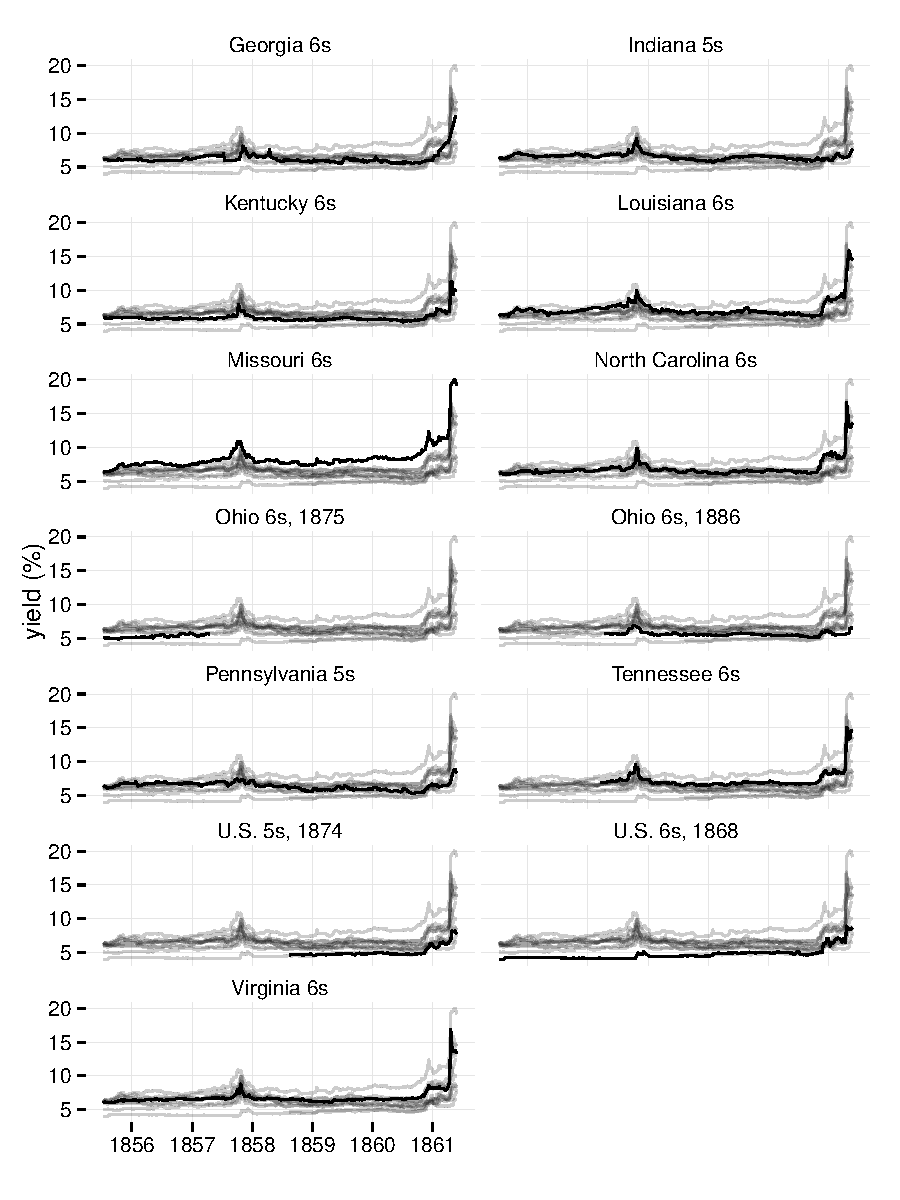
\includegraphics{figures/fig_yields_all-1}
\caption{Yields to maturity of U.S. government and state bonds, by bond, July  1, 1855 to June  1, 1861.}
\label{fig:yields_all}
\end{figure}


\begin{figure}
  \centerfloat
  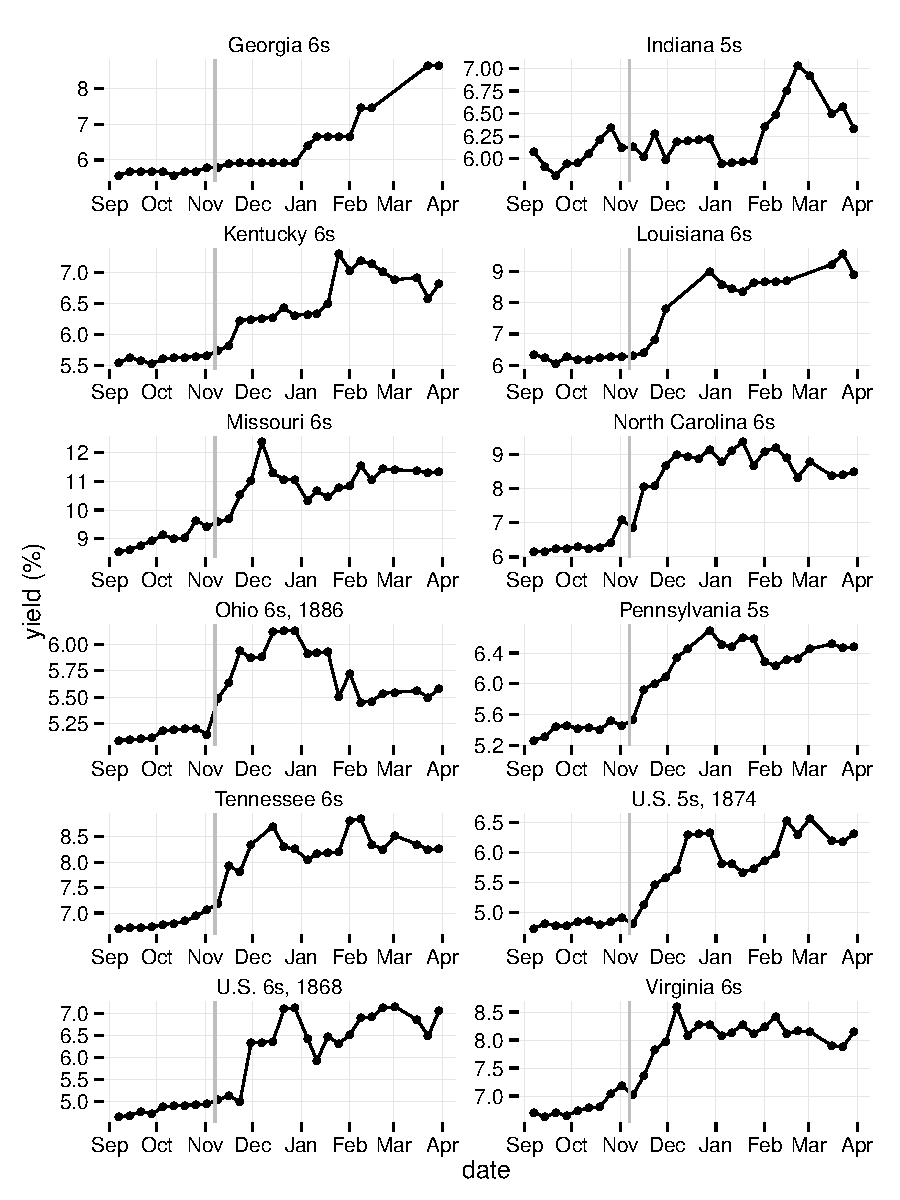
\includegraphics{figures/fig_yields_election-1}
\caption{Yields to maturity of U.S. government and state bonds before and after the election of 1860.
  The vertical lines indicate the date of the election, November 6, 1860.}
\label{fig:yields_election}
\end{figure}

\begin{figure}
  \centerfloat
  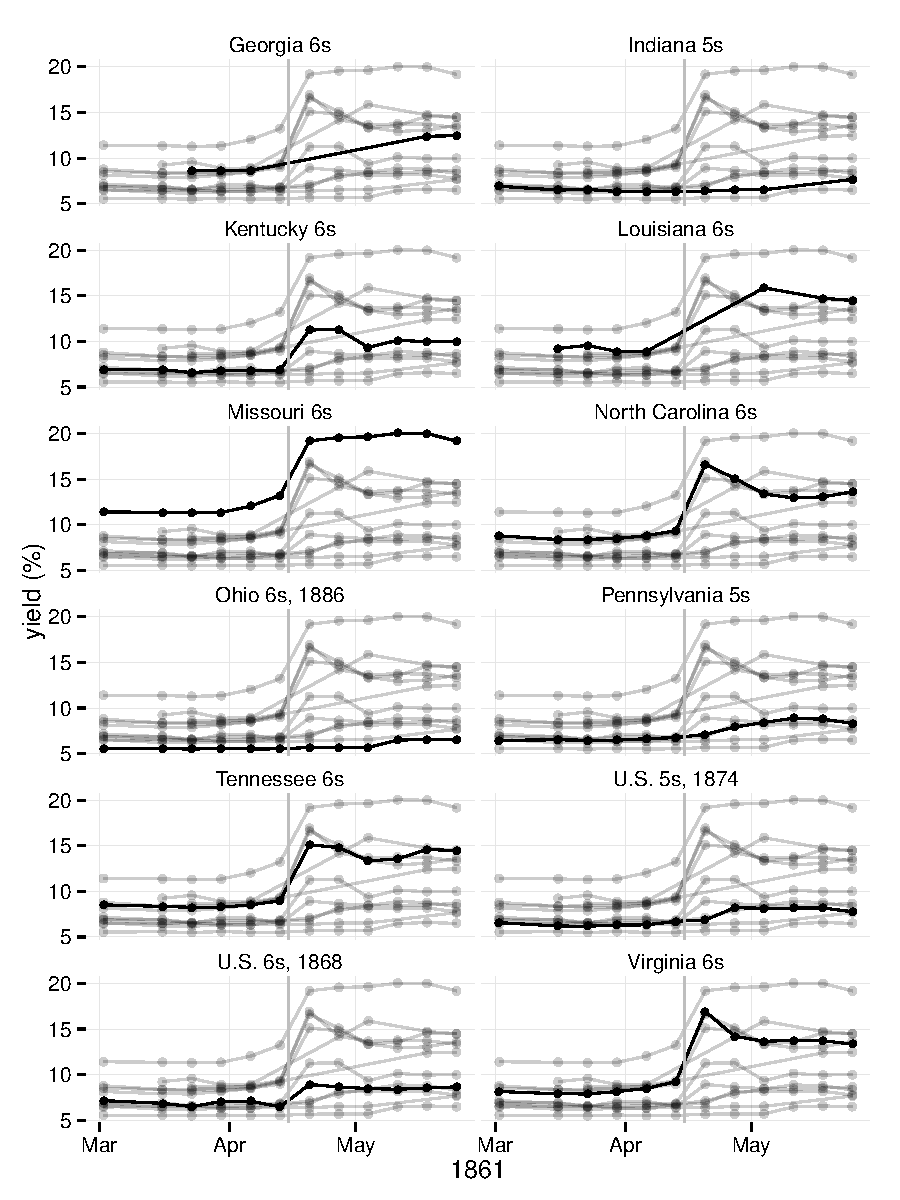
\includegraphics{figures/fig_yields_sumter-1}
\caption{Yields to maturity of U.S. government and state bonds before and after the Battle of Fort Sumter. The vertical lines indicate the date when news of the surrender of Fort Sumter reaches New York, April 15, 1861.}
\label{fig:yields_sumter}
\end{figure}

This section discusses the yield data of the U.S. government and state bonds discussed in the previous section.
The purpose of this section is to provide the reader and understanding of the data and the context to interpret the more specific measures of the risk of war, the spread between southern and northern state bonds and the implied proability of war, which will be presented in the following sections.

Figure~\ref{fig:yields_all} plots the yields of all the bonds in the data from July  1, 1855 to 1861-06-01.
By visual inspection, these time series can be divided into five periods:
July 1855 to October 1857,
November 1857 to January 1858 (the Panic of 1857),
February 1858-October 1860,
November 1860-April 14, 1861,
and after the start of the war with Fort Sumter (April 14, 1861).


From July 1855 through October 1857, yields were low and stable.
The yields of the U.S. 6s of 1868 were between 3.93 and 4.31 percent.
These were the lowest yields on U.S. government bonds up to that point \parencite[282-283]{HomerSylla2005}.
The yields were even lower than the traditionally safe Massachusetts and Boston city bonds, and less than one percentage point higher than the yield on 3\% British consols, which were considered the safest global asset during that period.%
\footnote{The average annual yields on British consols 1855-1857 were between 3.27 and 3.31 \parencite[193]{HomerSylla2005}.}
State bond yields were also relatively stable, although having higher yields than government bonds; with average yields between 5.29 (10) and 7.57 (8).
State bonds had higher yields than U.S. government because were perceived to be relatively riskier assets, since beween 1841 and 1842 nine states or territories defaulted on their debts \parencite{English1996}.%
\footnote{Of the states with bonds in the data, Indiana, Pennsylvania and Louisiana defaulted in the 1840s \parencite[265]{English1996}.}
%Although higher than government bond yields, the yields of the state bonds during this period were still much lower than the previous decade, when some states had yields of above 10 percent and as high as 41 percent \parencite[320]{HomerSylla2005}.
Overall, the relatively low and stable yields suggest that the market did not assign much, if any, risk to war.
% TODO: discuss Missouri. But would need to do structural break analysis.

From October 1857 to January 1858, yields spiked during the Panic of 1857.
The Panic of 1857 was a recession and financial crisis that included the failure of a major insurance company, the failures of banks and railroads, and the suspension of specie payments by banks in New York City.
The causes of the panic were not directly related to political risks of secession or war, but were likely a decline in European demand for U.S. trade or insufficient specie supply to meet demand due to a decline in gold production \parencites[263-265]{Dewey1918}[277,299]{HomerSylla2005}[337]{BankersMagazine1857}.
The \textit{Bankers' Magazine} ``Notes on the Money Market'' sections of the time do not mention domestic political issues during the Panic of 1857, attributing it to a decline in foreign trade and bad banking \parencite[337]{BankersMagazine1857}.
Thus, while yields reached high levels the panic, these high yields are almost certainly not attributable to an increase in war risk.

After the Panic of 1857, from February 1858 to November 1860, yields of bonds returned to levels similar to the period prior to the Panic of 1857.
While the yields of U.S. government bonds were also stable during this period, their yields were approximately 0.5 percentage points higher than they had been before the panic.
The yields of state bonds were also similar to or in some cases lower than in the period prior to the panic.

Lincoln's victory in the presidential election on November 6, 1860 precipitated a rise in yields, especially for southern state bonds.%
\footnote{Lincoln's victory was known the next day: ``It is too certain to speak confidently of detailed results of yesterday's elections. But there can be no reasonable doubt that the Republicans have elected their president.'' \parencite{NYT1860}}
The yields of bonds before and after the election are plotted in Figure~\ref{fig:yields_election}.
The market partially anticipated the political issues that would arise with Lincoln's election, as there was a slight increase in yields in October 1860.
This rise was partially due to a monetary contraction as the economy went into recession \parencite[413]{BankersMagazine1861}, but also the anticipation of a Republican victory in the election.%
\footnote{The U.S. was in a slight recession prior to the start of the American Civil War, from October 1860 to June 1861, according to the  \href{http://www.nber.org/cycles/cyclesmain.html}{NBER}.}
The \textit{Bankers' Magazine} described the market,
\begin{quote}
   The market for Government and State loans during the month has been dull.
   Prices have in most instances tended downward and a material decline is perceptible in some of the most prominent securities.
   The principal reasons for this seem to be the political excitement.  \parencite[414]{BankersMagazine1861}
\end{quote}
The market reaction was likley in response the Republican victory in the Pennsylvania gubernatorial election on October 9:
\begin{quote}
  The election in Pennsylvania early in October and the prospect which it gave of the election of the Republican candidate for President in November caused the timid to pause. ...
  The political complications of the day were the sole cause relied on by the bears and totally ignoring every other element in the market the pressure to sell under the influence of this sudden fear of some dreadful calamity became irresistible. ...
  The partisan presses aided the decline as far as they could and did their best to make it a panic by spreading abroad the most gloomy picture of the state of feeling at the South and directly prophesying ruin complete and full in the event of Mr. Lincoln's election.
  \parencites[476-77]{BankersMagazine1861}
\end{quote}
While the market believed it was likely that Lincoln would win the election and aware that Lincoln's election cause political risk, the  response observed in the yields was minimal.

It was not until after Lincoln's election that yields increased dramatically.
However, this increase did not occur immediately after Licoln's election victory, as would occur with Fort Sumter, but yields rose over the course of the following month, with some variation between bonds in the timing of the rise.
However, by the end of January 1861, southern and border state yields had increased 1--3 percentage points, and the yields on U.S. government bonds had increased 1--1.5 percentage points.
The initial increase in yields was due a small financial crisis that started when southern banks started denying credit to northern clients and withdrew specie from Northern banks \parencite[76]{HomansDana1861a}.
However, the response of banks mitigated the severity and duration of the crisis, and it was largely resolved by November \parencite[539-542]{BankersMagazine1861}.
However, political risk remained a concern:
\begin{quote}
\item The money market during December recovered somewhat from the worst effects of the panic.
  The action of the banks had been prompt and energetic, and the relief afforded by their largely expanded line of loans and discounts averted the worst consequences of the panic.
  The want of confidence in the political future prevented however a complete recovery and the results of prostrated credit and destroyed confidence were everywherfe discernable. \parencite[\textit{Bankers' Magazine}, January 1861:][541]{BankersMagazine1861}

  The only speck in the horizon is the threat of secession in the South.
  We would be the last to give countenance to the libel upon the South, that the majority of any one State assented to the proposition of secession.
  The permanent social, commercial and financial interest of the various sections of the whole country are too strongly identified---too strongly bound together---to induce the loss of any one State. \parencites[\textit{Bankers' Magazine}, December 1860:][419]{BankersMagazine1861}
\end{quote}
While yields increased during this period, the yields on most bonds were less than their peak during the Panic of 1857.

Many of the bond series appear continue rising until dates near the ordinance of secession by South Carolina on December 20, 1860.
In the months between the election and the start of the war, yields remained high, but also variable as they responded to political events \parencites[718]{HuntKettellHomansEtAl1860}[78,198,416,677]{HomansDana1861a}[413,481,669,756,838]{BankersMagazine1861}.%

Comparing the individual series of the southern state bonds, the market appeared to have treated the slave-holding states similarly, regardless of whether they had formally seceeded prior to the start of the war.
Although Louisiana did not seceed until January 26, its yield had already peaked near 9 percent at the start of January.
Virginia, Tennessee and North Carolina did not seceed until after the start of the war, yet the yields on all of these states rose between November and January.%
\footnote{Georgia is an exception; its yields noticeably increase after the election until January 1861 near is declaration of secession (January 19, 1861).
This may be because the Georiga 6s were illiquid; in the data, there are long sequences in which the price of the Georgia bonds does not change, and it is often traded in multiples of 5 or 10.
}

Although bond yields had risen after the election of Lincoln as the risk of civil war increased, the formal start of the war with the Battle of Fort Sumter was followed by a jump in yield much larger than had been observed after the election or during the Panic of 1857.
The start of the war resulted in a `` depreciation in Southern State stocks exceeding any decline ever witnessed at the stock board of this city.quantifying uncertainty'' \parencite[919]{BankersMagazine1861}.
Unlike the election of 1860, in which bond yields rose over a period of weeks, prices fell and yields increased immediately after news of Fort Sumter reached the market.
Figure~\ref{fig:yields_sumter} plots the yields around the Battle of Fort Sumter (March--June 1861).
Table~\ref{fig:yields_sumter} tabulates yields in the week immediately before and after news of the surrender of Fort Sumter reached the New York market.
Southern state yields rose between 6.1 (Tennessee) and 7.7 (Virginia) percentage points (41 and 45 percent) between April 13th and 20th.
The yields of U.S. sixes also fell, but only by 2.5 percentage points,
while northern state bond yields were almost unchanged.%
\footnote{The price of the U.S. 5's of 1874 did not change noticeably until the following week, April 27, 1861}
Since the yield of the bond incorporates expectations about future payoffs and war would certainly affect those payoffs, the extreme rise in yields after Fort Sumter imply that the probability the market assigned to war was low.
It is likely that even on the eve of the war, the market anticipated some sort of peaceful settlement to the crisis.
In April 1860, \textit{The Bankers' Magazine} wrote, ``The general condition of commercial and financial affairs still turns upon the uncertain political future. The fears of civil war, that at one time were entertained in certain quarters, have subsided, if not altogether disappeared, under the influence of passing events.'' \parencite[413]{HomansDana1861a}
while \textit{The Merchants' Magazine} wrote,
\begin{quotation}
  The securities of the Border States fluctuate from day to day as the tone of dispatches from Washington leans toward peace or war.
  There is undoubtedly a great want of confidence as to the final course which those States will pursue and it is the strong hope which is entertained of their remaining loyal which alone keeps up their price. \parencite[838]{BankersMagazine1861}
\end{quotation}
The magnitute and speed of the reaction of yields with respect to the Battle of Fort Sumter implies that the markets' hope that southern states would remain loyal, must have been very strong.
The reaction of the market to the Battle of Fort Sumter also implies that the market considered it the start of hostilities, even though large-scale engagements would not occur for months with the First Battle of Bull Run

\section{South-North Yield Spread}
\label{sec:south-north-yield}


\begin{figure}
  \centerfloat
  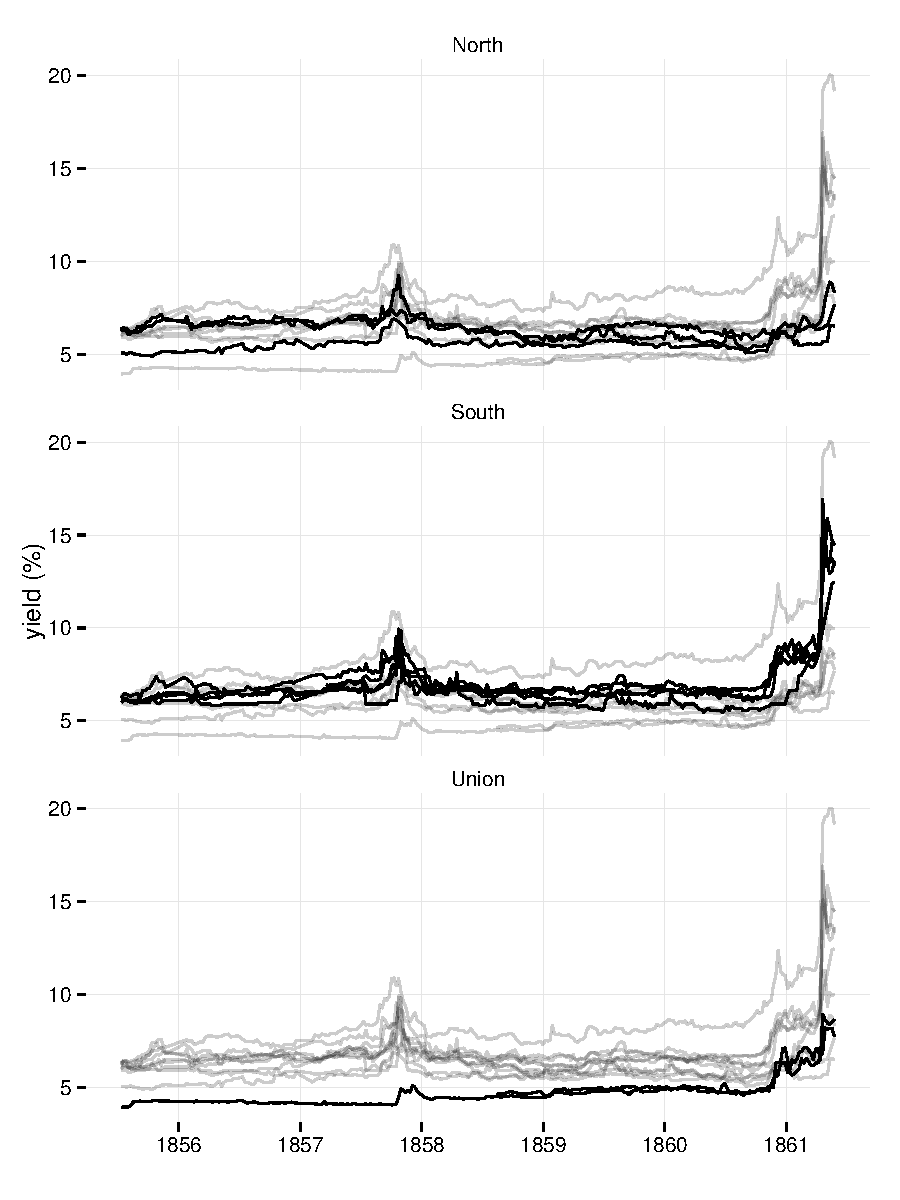
\includegraphics{figures/fig_yields_regions-1}
\caption{Yields of U.S. government and state bonds, by region, July  1, 1855 to June  1, 1861.}
\label{fig:yields_regions}
\end{figure}

\begin{figure}
  \centerfloat
  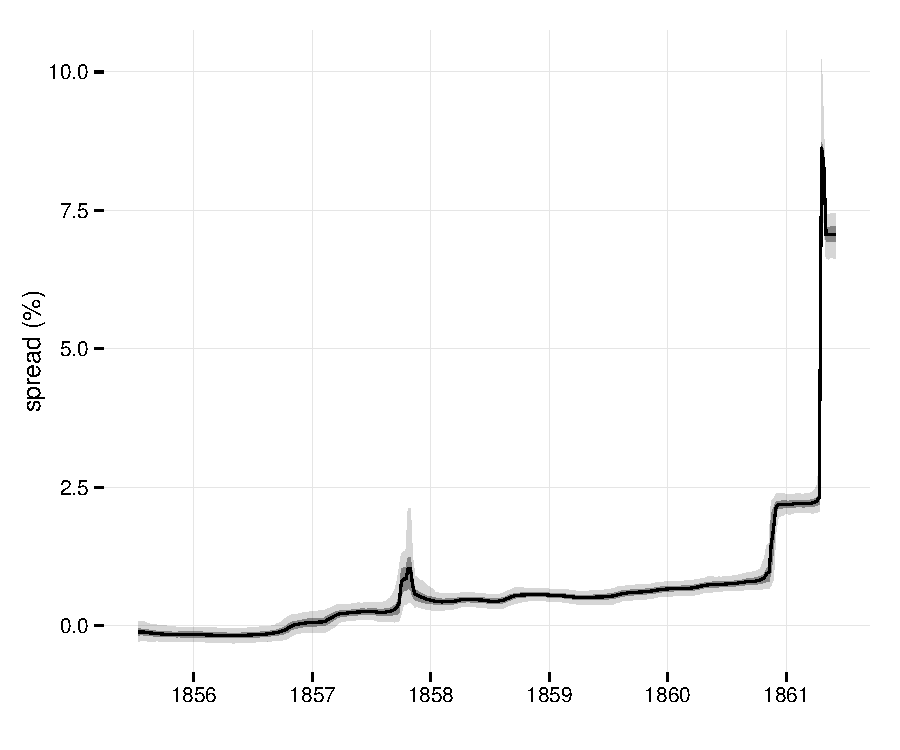
\includegraphics{figures/fig_north_south_spreads-1}
\caption{
  Estimated spread between the yields of southern and northern state bonds.
  The line is the posterior mean, the dark ribbon is the 50\% credible interval, the light ribbon is the 95\% credible interval.
}
\label{fig:north_south_spreads}
\end{figure}

For the case of the American Civil War, the spread (difference) between the average yield of the southern and northern state bonds is a measure of the market's expectation of war.%
\footnote{
  The spread between southern and northern bonds is approximately the difference in default risk between the bonds, when the recovery rate is 0.
  This follows from Equation~\eqref{eq:4}.
}
An increased risk of war increases the spread between southern and northern bond yields, because war would make southern state bonds relatively more risky than northern state bonds.
Although war could increase the riskiness of all state bonds, there are at least two ways in which war would increase the risk of southern bonds relative to northern state bonds.
First, and most immediately, southern states would immediately stop the payment of interest to northern investors at the start of conflict.
As dicussed in section~\ref{sec:risky-bond-pricing}, the suspension of interest did happen and was anticipated by investors.
Second, less immediately, it is likely that a war would be fought primarily in southern states, and thus southern states would incur more destruction that could hinder their ability to repay debt in the future.%
\footnote{In the estimates of the economic cost of the American Civil War in \textcite{GoldinLewis1975}, physical capital loss was the largest component of the direct cost of the war to the Confederacy \parencite[308]{GoldinLewis1975}}
The differential effect the war on the risk of southern and northern bonds was observed in the changes in the yields of these bonds after the Battle of Fort Sumter, as shown in Table~\ref{tab:sumter}.
In the week after after Fort Sumter, the yields of southern states increased 3--8 percentage points, while the yields of northern states increased only 0.01 to 0.35 percentage points.
An advantage of using the spread rather than the yields of each bond, is that it controls for shocks affecting all state bonds as well as averaging over idiosyncratic shocks to individual states.
There can still be regional differences in the risk of southern and northern state bonds due to factors other than war risk.
However, focusing on changes in the spread rather than the level of the spread controls for any of these regional factors which are constant over the time period considered.

The data used to calculate the south-north yield spread consists of the yields of northern (Indiana, Ohio and Pennsylvania) and southern (Georgia, Louisiana, North Carolina, Tennessee and Virginia).
\footnote{The border states of Kentucky and Missouri are not included in these calculations.}
Let $y_{j,t}$ be the yield for bond $j$ at time $t$.
The yield for each bond is modeled as,
\begin{equation}
  y_{j,t} \sim \dt{\nu}{\theta_{t} + \psi_{t} \mathtt{south}_{j}, \sigma}
\end{equation}
where $\dt{a}{b, c^{2}}$ is the Student's $t$-distribution with degrees of freedom $a$, location $b$ and scale $c$, and
$\mathtt{south_{j}}$ is a binary variable indicating whether the bond was issued by a southern state.

Since the number of bonds in each period is relatively small, the parameters $\theta$ and $\psi$ are smoothed over time with random walk priors.
However, the method used to pool rates over time cannot overly smooth the data since, otherwise the method would obscure the effect of important events on the spread.
In order to achieve behavior similar to a change-point model, this paper uses a shrinkage prior for the first difference of $\psi$ and $\eta$.
Shrinkage priors are the Bayesian equivalent to penalized estimate like lasso \parencites{Tibshirani1996}{ParkCasella2008}.
The particular shrinkage prior employed horseshoe prior distribution is used \parencites{CarvalhoPolsonScott2009}{CarvalhoPolsonScott2009}.
The horseshoe prior has properties similar to a spike-and-slab prior while being continuous.
This is similar to estimating change points in the parameter, while estimating the number of changepoints from the data.
\footnote{This approach is similar to a Baysian version of the fused lasso \textcite{TibshiraniEtAl2005} using the horseshoe prior distribution rather than a Laplace distribution for the reasons discussed in \parencites{CarvalhoPolsonScott2009}{CarvalhoPolsonScott2009}.}
\begin{align}
  \theta_{t} & \sim \dnorm{\theta_{t-1}, \sigma^{2} \tau_{\theta}^{2} \lambda_{\theta,t}^{2}}
  & \lambda_{\theta,t} & \sim \dhalfcauchy{0, 1} \\
  \psi_{t} & \sim \dnorm{\psi_{t-1}, \sigma^{2} \tau_{\psi}^{2} \lambda_{\psi,t}^{2}}
  & \lambda_{\psi,t} & \sim \dhalfcauchy{0, 1}
\end{align}
where $\dnorm{N}{a, b^{2}}$ is the normal distribution with mean $a$ and scale $b$, $\dhalfcauchy{0, a}$ is the half-Cauchy distribution with scale $a$.%
\footnote{Note that variable and parameter names are only unique for this section; variables and parameters with the same name in different sections do not necessarily correspond to the same thing.}
In summary, this set of priors method attempts to estimate the parameters, e.g. $\theta$, where the first differences, $\theta_{t} - \theta_{t-1}$, are sparse (mostly zero) while not imposing assumptions about the sparsity of the differences.
The model is estimated using Bayesian methods.
The posterior distribution is sampled with the No-U-Turn Sampler implemented in Stan \parencites{Stan2014}{HoffmanGelman2013}.

Figure \ref{fig:north_south_spreads} plots estimates from the posterior distribution of the south-north spread ($\psi_{t}$) for all periods.
For most of the period, the spread was positive, meaning that southern state bonds were riskier on average than northern state bonds.
The spread is increasing over most of the period before settling down immediately before the election.
Between the start of the period (July 1, 1855) and prior to the election of 1860 (November 2, 1860), the spread increased by 1.06 (0.73, 1.45),
from -0.11 (-0.28, 0.08) to 0.95 (0.68, 1.45).
The spread increased even though the yields of southern bonds remained largely stable or even slightly declined, because the yields of northern bonds, especially Indiana and Pennsylvania, declined much more.
The Panic of 1857 has some effect on the spread, but less than for the yields, and the uncertainty in the estimated spread increases during that period.
The spread increases sharply after the election of Lincoln, from November 2, increasing by 1.23 (0.7, 2.4) percentage points to 2.18 (1.95, 2.4) on December 7, 1860.
The spread is stable until the the Battle of Fort Sumter, when it increases 6.31 (5.47, 7.88) percentage points to 2.32 (2.07, 2.91).

Thus the risk of southern bonds relative to northern bonds was increasing over the period, perhaps due to increasing assessements of the risk of war.
The markets' beliefs about the risk of war jumps after Lincoln's election, but the jump in spreads is about 5 times smaller than the spread that is observed after war did start.

\section{Probability of War}
\label{sec:probability-war}


While the bond yields and spreads between northern and southern bonds can indicate changes in war risk, they are not directly interpretable as the probability of war.
However, the market's beliefs about the probability of war can be inferred from bond prices and yields by treating war as a default event \parencite{HaberEtAl2012}.%
\footnote{See \textcites{Fons1987}{Merrick2001}{Chan-Lau2006} for derivations of default probabilities from bond prices.}
A simple approximation for the probability of risk-netural default probability per year of a risky bond given its yield is,
\begin{equation}
  \label{eq:4}
  \Pr(\text{default}) = \frac{y - r}{1 - R} \text{,}
\end{equation}
where $y$ is the yield of the risky bond, $r$ is the yield of a risk-free bond with comparable cashflows, and $R$ is the the recovery value of the bond in the event of the default as a proportion of the face value of the bond \parencite{HullPredescuWhite2004}.%
\footnote{\textcite[115]{WaldenstromFrey2008} propose a similar method, that when the war is observed the probability of war is the proportion of the yield after war to the yield prior to war.
  That method is not directly derived from a cashflow model and produces higher estimates of the pro*bability of war.
  \textcite{HaberEtAl2012} use a cashflow method to calculate the probability of victory in wars (Confederate victory in the American Civil War, and government victory in the Chinese Civil War) using a cashflow pricing model of bonds, but assuming a recovery rate of 0.
}
Equation~\eqref{eq:4} can be used to estimate the probability of war if $r$ and $R$ are properly defined.

When estimating the probability of war, the risk-free interest rate $r$ should be defined to be the yield of a comparable bond with no risk of war.
In this case, $r$ will not necessarily be risk-free --- it should include any risk not due to war, but exclude risk due to war.
This work will use is the yield of the same bond for an earlier period in which the risk of war is approximately as $r$.

The recovery rate $R$ is the amount, as a proportion of par value, that the investor receives in the event of a war.
If war does occur, then the value of $R$ to use is straightforward because it is known --- it is the price of the bond observed at the start of the war.
 method The implied probability of war is calculated for all southern and border state bonds (Georgia, Kentucky, Louisana, Misosuri, Tennessee and Virgia)
For each bond $j$, the implied probability of war at time $t$, $\pi_{t}$, is
\begin{equation}
  \pi_{t} = \frac{y_{j,t} - r_{j}}{1 - R_{j,t}}
\end{equation}
For each bond, $r_{j}$ is its average yield from July  1, 1855 to September  1, 1857.%
\footnote{
  The Panic of 1857 (August 1857 through January 1858) is excluded from calculations because as discussed earlier in this paper, while the yields increased during this period, it was due to a financial crisis and not war risk.
}
Although there may have been some risk of war during this period, the yields were low (see section \ref{sec:yields-governm-state}), and thus it is unlikely that war risk could not have been high.
While this estimate of the war-risk free rate accounts for the risk hetereogeneity between the bonds, it makes the strong asusmption that $r_{j}$ is that it is constant over time.
Since it does not allow the war-risk free rate to vary over time, the estimates of the probability of war can be confounded by any factors which affect $r$.
In order to reduce this possibility, I only consider the period between the Panic of 1857 and the Battle of Fort Sumter, when there are no major non-war financial crises and changes in war risk are most likely.

For each bond, the value of $R_{j,t}$ is the approximately the price of the bond immediately after the Battle of Fort Sumter.
More precisely, the $R_{j,t}$ is the present value of bond $j$ at time $t$ calculated using the average yield of the bond April 15, 1861 to May 18, 1861.%
\footnote{The average yield is used since the prices of most bonds spiked after Sumter before falling somewhat in the weeks after it.
  Using the average yield rather than the first observation after Sumter gives a less conservative estimate of war.
}
The value of $R$ incorporates expectations about the financial risk posed by expected course of the war, which is key to allowing separating the war risk due to the probability of war and the risk war will have on the bond, conditional on war occuring.%
\footnote{
  An implicit assumption in these calculations is that expectations about the costliness of the war were constant prior to the start of the war and only beliefs about the probability of a war was changing in the periods leading up to the war.
  In the case of the American Civil War, this seems like a reasonable assumption.
}

Figure~\ref{fig:prwar1} displays the implied probabilities of war for each bond calculated with Equation~\eqref{eq:4}.
There are three things to note about the implied probabilities in that figure.
First, the implied probability of war is approximately 0 for all bonds prior to the election of Lincoln in 1860.
Second, although the implied probabilities increase to between 3 and 5 percent.
Third, the implied probabilities largely agree, but there are differences in the probility of war implied by each bond.

By noting that all the implied probability of war should be the same for all bonds, rearranging \eqref{eq:4} and adding uncertainty, the probability of war in each time period can be estimated as,
\begin{align}
  \label{eq:1}
  \log y_{j,t} & \sim \dnorm{(1 - R_{j}) \pi_{t} + r_{j}, \sigma^{2}}
\end{align}
where $\pi_{t}$ is the probability of war at time $t$,
Equation~\eqref{eq:1} is a regression model with time-varying coefficients ($\pi_{t}$).
The inverse logit transformation of $\pi$ evolves as a random walk with a horseshoe prior on the innovations to allow for change-points, as desribbed  in section~\ref{sec:south-north-yield}:
\begin{align}
  \pi_{t} &= \logit^{-1}(\theta_{t}) \\
  \phi_{t} &\sim \dnorm{\phi_{t-1}, \tau^{2} \lambda_{t}^{2}} \\
  \lambda_{t} &\sim \dhalfcauchy{0, 1}
\end{align}
%% Since the war-risk free interest rate of the bonds are uncertain:
%% \begin{align}
%%   r_{j} & \sim \dnorm{\bar{r}_{j},s_{j}}
%% \end{align}
%% where $\bar{r}_{j}$, $s_{j}$ are the mean and standard deviation of the logarithm of yields for bond $j$ for the period, DATEFMT_PEACE_START  to DATEFMT_PEACE_END.

The estimated values of $\pi_{t}$ from the previous are plotted in Figure~\ref{fig:prwar2}.
The probability of war is estimated to be approximately 0 prior to Lincoln's election.
After the election, the probability of war rose to 2.5 (2.1, 2.8) percent by January 5, 1861,
to 3 (2.6, 3.4) percent on February 8, and to 4.1 (3.3, 4.9) on April 13, days before news of the outcome of the Battle of Fort Sumter reached the market.

These results are largely consistent with the results in section~\ref{sec:south-north-yield}.
The market estimated that war was almost certainly not likely prior to the election of Lincoln.
Only after the election did the market adjust its estimates of the risk of war.
However, even immediately before the war, the probability of war was estimated to be highly unlikely; while the measures of the previous section did not provide a direct estimate of that probability, this measure in this section does.
The results differ in that although both measures show little risk of war prior to the election of Lincoln, the estimates south-north yield spread show an increasing risk of war over time, while the implied probability of war from this section show that risk constant at 0.
This difference likely arises from the use of a constant war-risk free rate in equation~\eqref{eq:1}.%
\footnote{This could be avoided if a good time-varying estimate of the war-risk free interest rate were available.
  Currently available data of the risk free interest rate of the era are only available at low frequencies: prior to 1857, the yields of Massachusetts 5s and Boston City bonds are only available at a yearly frequency prior; after 1857, an index of New England state and municipal bonds is avaiable at a quarterly frequency \parencite{Officer2003}.
  Using the average of northern state bonds, as in section~\ref{sec:south-north-yield}, is likely inappropriate because they also include some risk of war.
}
Nevertheless, the overall pattern between the results is similar.

\begin{figure}
  \centerfloat
  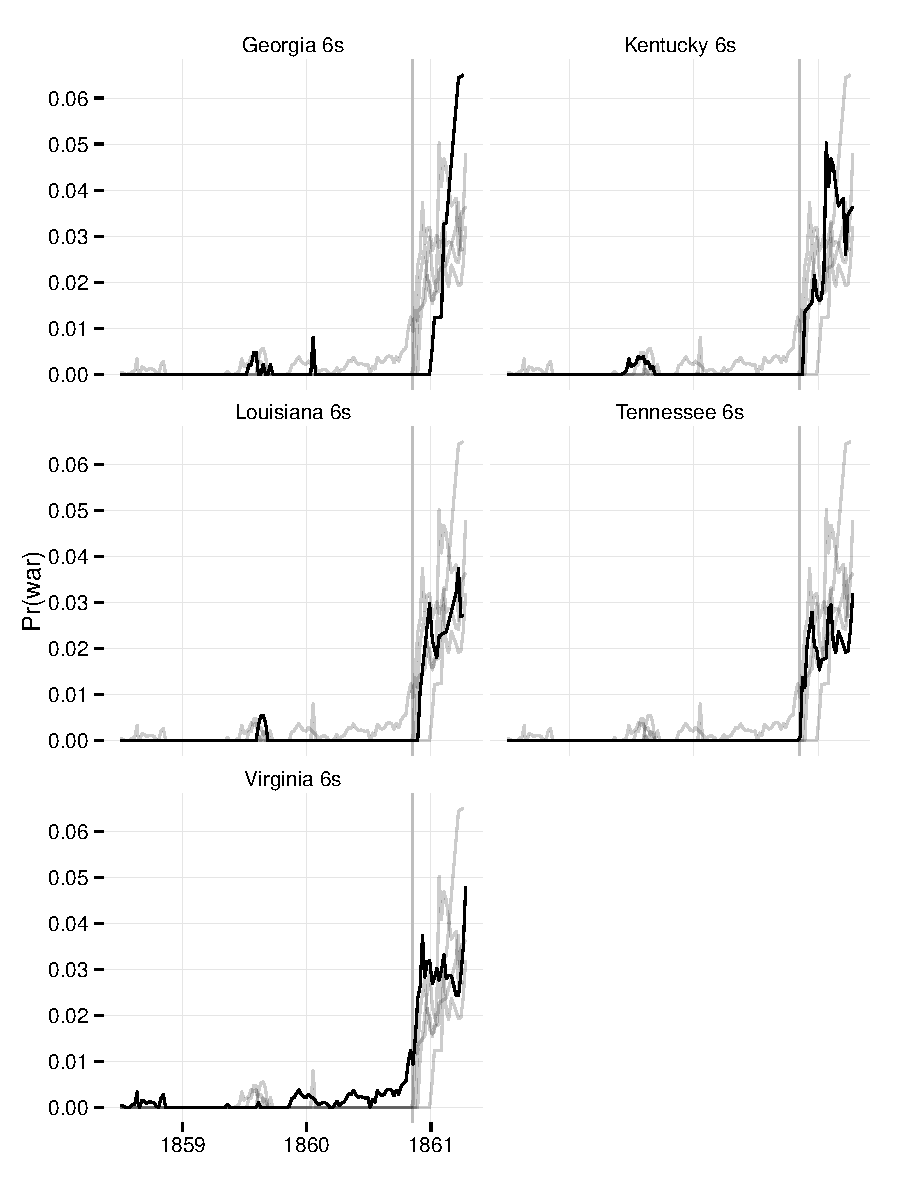
\includegraphics{figures/fig_prwar1-1}
  \caption{Implied probabilities of the initiation of war calculated from southern and border state bonds, March  5, 1858 to April 13, 1861.}
  \label{fig:prwar1}
\end{figure}

\begin{figure}
  \centerfloat
  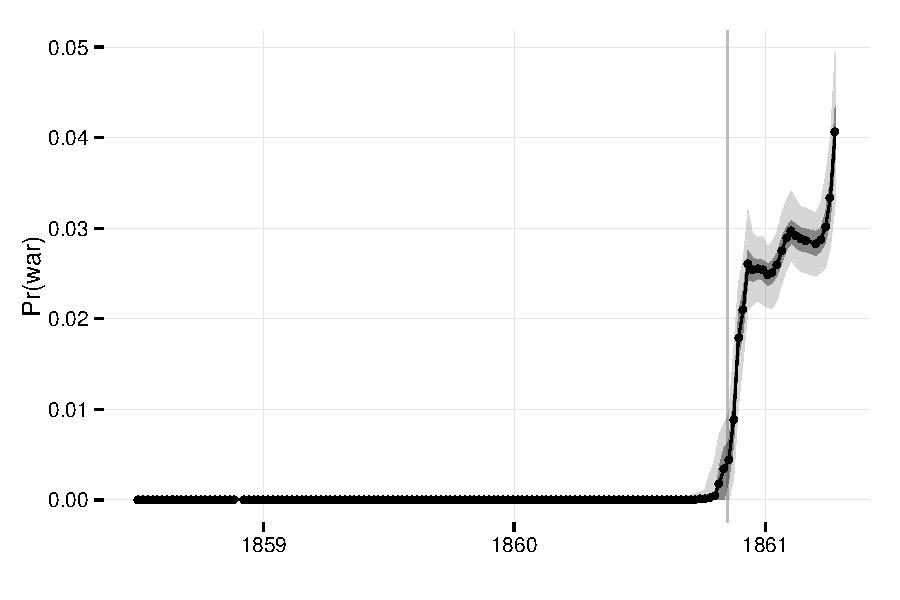
\includegraphics{figures/fig_prwar2-1}
  \caption{
    Implied probabilities of the initiation of war calculated from U.S. government and southern and border state bonds, March  5, 1858 to April 13, 1861, using the model described in section \ref{sec:probability-war}
    The line is the posterior mean, the dark ribbon is the 50\% credible interval, the light ribbon is the 95\% credible interval.
    The vectical line is the date of Lincoln's election.
  }
  \label{fig:prwar2}
\end{figure}

\begin{table}
  \centerfloat
  % latex table generated in R 3.2.2 by xtable 1.7-4 package
% Mon Oct 19 12:58:41 2015
\begin{tabular}{rrrrr}
  \hline
 & \parbox{2.5cm}{\raggedleft Avg. yield \\ 1858-02-01--\\1860-11-07} & \parbox{2.5cm}{\raggedleft Avg. yield \\ 1860-11-07--\\1861-04-15} & \parbox{2.5cm}{\raggedleft $r$\\ Avg. yield \\ 1855-07-01--\\1857-09-01} & \parbox{2.5cm}{\raggedleft $R \cdot 100$ \\ Avg. price \\ 1861-04-15--\\1861-05-18} \\ 
  \hline
Georgia 6s & 5.92 & 6.72 & 6.15 & 62.52 \\ 
  Kentucky 6s & 5.68 & 6.59 & 5.86 & 74.60 \\ 
  Louisiana 6s & 6.70 & 8.31 & 6.90 & 48.00 \\ 
  Tennessee 6s & 6.76 & 8.30 & 7.13 & 43.85 \\ 
  Virginia 6s & 6.50 & 8.12 & 6.48 & 43.65 \\ 
   \hline
\end{tabular}

\caption{Summary of data used to calculate probability of war}
\label{tab:prwar1}
\end{table}

\section{Conclusion}
\label{sec:conclusion}

This work estimates the
Although the seeds of the American Civil War were preceeded the start of the war for many years, the onset of war was unexpected by financial markets.
Financial markets did not respond to war risk until after the election of Lincoln in November 1860, and then only after a financial criss due to southern banks withdrawing specie and discussion of secession became srioues.
Despite the awareness of the risk of war, yields spiked dramatically after the Battle of Fort Sumter, implying that the event was unanticipated.
The implied probability of war based off the southern state bonds was only about 5 percent.

The results presented here are specific to the case of the American Civil War, but they are consistent with other work on how financial markets have responded to war initiation.
\textcite{Ferguson2006} show that although World War I was preceeded by a series of crises, European markets did not anticipate the onset of WWI.
\textcite{FreyKucher2000} and \textcite{WaldenstromFrey2008} show that Nordic and Swiss markets had large reactions to the start of World War II although this was known.
\textcite{GuidolinLaFerrara2010} find large abnormal returns at MIDs.
Many of those works emphasize the efficiency of markets in responding to political events, or use the size of the market reaction to understand characteristics of the political events.
However, the presence of strong market reactions to these events it itself interesting, as it is an indication that the onset of hostilities was unexpected.
Overall, These cases suggest in in many cases financial markets do not effectively price in the the risk of war.
If markets are efficient and incorporate public information, this suggests that given public information, many wars are not anticipated.
Alternatively, markets do a poor job of assessing the \textit{ex ante} theory of war.
Either of these scenarios have important implications for prominent theories of war.

The \textit{ex ante} public information assessments of the probability of war are important because they may provide methods for distinguishing between theories and mechanisms of war.
The two rationalist theories of war: commitment problems and private information \parencites{Fearon1995,Powell2006}, have different implications as to what the \textit{ex ante} probability of war occuring will be.
In the simplest version of war due to a commitment problem, given the conditions, war will either occur or not occur with certainty depending on the parameters of the model.
However, in a private information model of war, if is is possible for war to occur, it can occur with a probability of less than one.
Not only that, the private information model of war implies that many wars should be unanticipated \parencite{Gartzke1999}.
In general, the prevalance of unanticipated wars would provide evidence for the prevalence of some sort of private information model.
Other more specific theories of war may offer different implications as to what the \textit{ex ante} probability of war would be.
However, the point remains that market predictions of war probability are both something to be explained by models of war, and a means to assess those models.
In the specific case here, the low probability of war implied by financial markets for the American Civil War is surprising given that several political science  explanations of the American Civil War emphasize commitment problems \parencite{Reiter2009}{Weingast1998}.

The second possibility is that financial markets maybe doing a poor job assessing and signaling the risk of war.
This would pose serious problems for the mechanism in the \textit{capitalist peace}.

This paper estimates the \textit{ex ante} risk of the American Civil War as implied by financial markets.
It is a single case, although its results of a low implied probability of war are largely consistent with other work on the reactions of financial markets to war.
The reactions of financial markets provide another empirical pattern that should be assessed with respect to theories of war.
In particular, if financial markets can serve as predictions given civil war, they provide a means to assess bargaining theories of war.

\newpage


\printbibliography{}


\end{document}

%%% Local Variables:
%%% coding: utf-8
%%% mode: latex
%%% TeX-engine: xetex
%%% End:

%  LocalWords:  ceteris parabis von Gartner Fearon FilsonWerner UCDP
%  LocalWords:  Slantchev SmithStam LeventogluSlantchev Goemans CDB
%  LocalWords:  LangloisLanglois WolfordReiterCarrubba Reiter Tierney
%  LocalWords:  SarkeesWayman cdb BiddleLong ACLED ESOC NorthWeingast
%  LocalWords:  RaleighLinkeHegreEtAl introd FreyKucher sussman revol
%  LocalWords:  instit Herron eldor finan chensiems Greenstone Schwab
%  LocalWords:  WolfersZitzewitz ArrowForsytheGorhamEtAl Calomiris th
%  LocalWords:  WillardGuinnaneEtAl McCandless SmithSmith Weidenmier
%  LocalWords:  BurdekinLangdana DavisPecquet BrownBurdekin kalyvas
%  LocalWords:  OosterlinckWeidenmier multimanned MarshallJaggers CBO
%  LocalWords:  BoltZanden GoldinLewis Poast Livermore dewey Godfrey
%  LocalWords:  HomerSylla annum ustreasury tri findata github eq HMC
%  LocalWords:  HoffmanGelman stan mcmcdb MCMC CWSAC ACWARD Phister
%  LocalWords:  Bodart KennedyConservation cwsac dbpedia Opequon Fons
%  LocalWords:  superpopulation Spotsylvania Proquest tuple Lau hoc
%  LocalWords:  macaulay DurbinKoopman Chickamagua ARIMA Reiter2003
%%  LocalWords:  Powell2006 GartzkeLi2003 Mitchell1903 McCandless1996
%%  LocalWords:  WillardGuinnaneEtAl1996 SmithSmith1997 Hall2004
%%  LocalWords:  BrownBurdekin2000 Weidenmier2002 WaldenstromFrey2008
%%  LocalWords:  LeighWolfersEtAl2003 WolfersZitzewitz2009 cashflow
